Twenty years ago, a computer with only one single processor may be considered as computing platform and be included in the Top 500 ranking of super computers. Nowadays, computing platforms have greatly evolved. Their architectures became more complex and varied. For this report, we propose here to distinguish them into four models. First, the \textbf{shared memory multi-cores} architecture, it is a computing platform consisting many cores and all have access to the same virtual memory. The \textbf{distributed memory} architecture is composed of at least two node. Each node has its own cores and its physical memory. Cores of different nodes cannot access to the virtual memory of each other, and thus, must communicate to share data. Even if in a distributed memory architecture, a node can consist many cores,  we will use - in this paper - the denomination \textit{distributed memory architecture} only for nodes with one single core. In contrast to the \textbf{hierarchical architecture} which is a distributed memory architecture where at least one node is a shared memory multi-cores architecture. Moreover, the \textbf{heterogeneous architecture} is a distributed memory architecture where at least one node is a GPU.

\section{Runtimes}
The most popular method to implement parallel distributed memory programs consists of using messaging systems. There are several different types of these systems such as message-passing like Message Passing Interface (MPI)\cite{Message94}. To achieve good performance with MPI, the knowledge of the whole architecture used is often advised. Moreover, the portability of performance is not always ensured. There is another type of messaging systems which tries to resolve these problems: the active-message, Charm++ is based on \cite{KaleLVandK1993b}.

In order to ease efficient use of supercomputers and to introduce an abstraction to computers architectures, the task flow model was used to implement other runtimes. In fact, task flows can be represented as a Direct Acyclic Graph (DAG) where vertices are tasks and edges are the dependencies between them. These runtimes schedule tasks on different nodes and move data according to tasks dependencies.
We propose here to distinguish runtimes based on task flow model into two families: those which run codes with implicit data dependencies and those which run codes with explicit data dependencies.

In order to ease the use of parallelism, while keeping the traditional way of programming, some runtimes run on codes with implicit data dependencies. These runtimes need only a set of tasks and their data access modes (read, write or read-write). With this information, the runtime extract the data dependencies and then build the corresponding DAG of task flow. Implementing parallel application over these runtimes is very similar to sequential codes. Quark implement this model for shared memory machines and is used in the Parallel Linear Algebra for Scalable Multi-core Architectures (PLASMA) library \cite{1742-6596-180-1-012037}.
StarSs is a collection of runtimes which can run on different types of architectures: CellSs for the Cell BE\cite{Bellens06}, SMPSs is for SMP architecture \cite{journals/concurrency/BadiaHLPQQ09}, and GPUSs for GPU \cite{Ayguade09}. In order to gather all types of architectures, StarPU is a unified runtime system that offers support for heterogeneous multicore architectures (GPGPUs, IBM Cell, ...). StarPU manage tasks execution through different architectures thanks to its data coherency protocol \cite{DoBiBo07,journals/concurrency/AugonnetTNW11}.


On the other hand, there are some runtimes based on explicit data dependencies by using Parametrized Task Graph (PTG).
Thanks to explicit data dependencies, these runtimes may benefit from efficient graph traversals. Moreover, PTG allow for compact representations of algorithms and induce a low overhead. Intel CnC is one of these runtimes dedicated - for the moment - to shared memory computers. \dague (Direct Acyclic Graph scheduler Engine) is also a runtime based on explicit data dependencies which can run on computers with shared and/or distributed memory.

In the rest of the paper, we focus on runtimes using explicit data dependencies. To illustrate the benefits on hierarchical computers (\ref{platform}), we will use the \dague runtime system. 
%We will also use StarPU for heterogeneous computers (\ref{platform}).

\section{LU Decomposition Algorithm}\label{lu_algo}
The LU decomposition algorithm is based on the Gauss elimination method and consists of factorizing a matrix into a product of a lower and an upper triangular matrix. In order to obtain a good accuracy, the swaps are - most of the time - needed. There is a lot of heuristic to perform the swapping, the most used by the scientist community is the partial pivoting for its practical stability and accuracy \cite{Hig02}, it is also used in the LINPACK benchmark which is used to rank the TOP 500 super-computers.

To illustrate an example of LU decomposition, we consider a $n*n$ square matrix. In order to benefit from efficient cache effects, state of the art dense linear algebra libraries implement a block version of the factorization. The matrix is split in $n_p$ block columns - so called panels - of $n_b$ columns ($n = n_p * n_b$). The (right looking) factorization of the matrix consists in a sequence of $n_p$ twofold operations. Indeed, at each step $p$ ($0 \leq p < n_p$), panel $p$ is factorized and the trailing sub-matrix is then updated. Figure \ref{fig:matrix} shows an example of matrix in the second step of the LU decomposition, the second panel is still being factorized, and after, the trailing sub-matrix will be updated.

\begin{figure}[!ht]
\centering
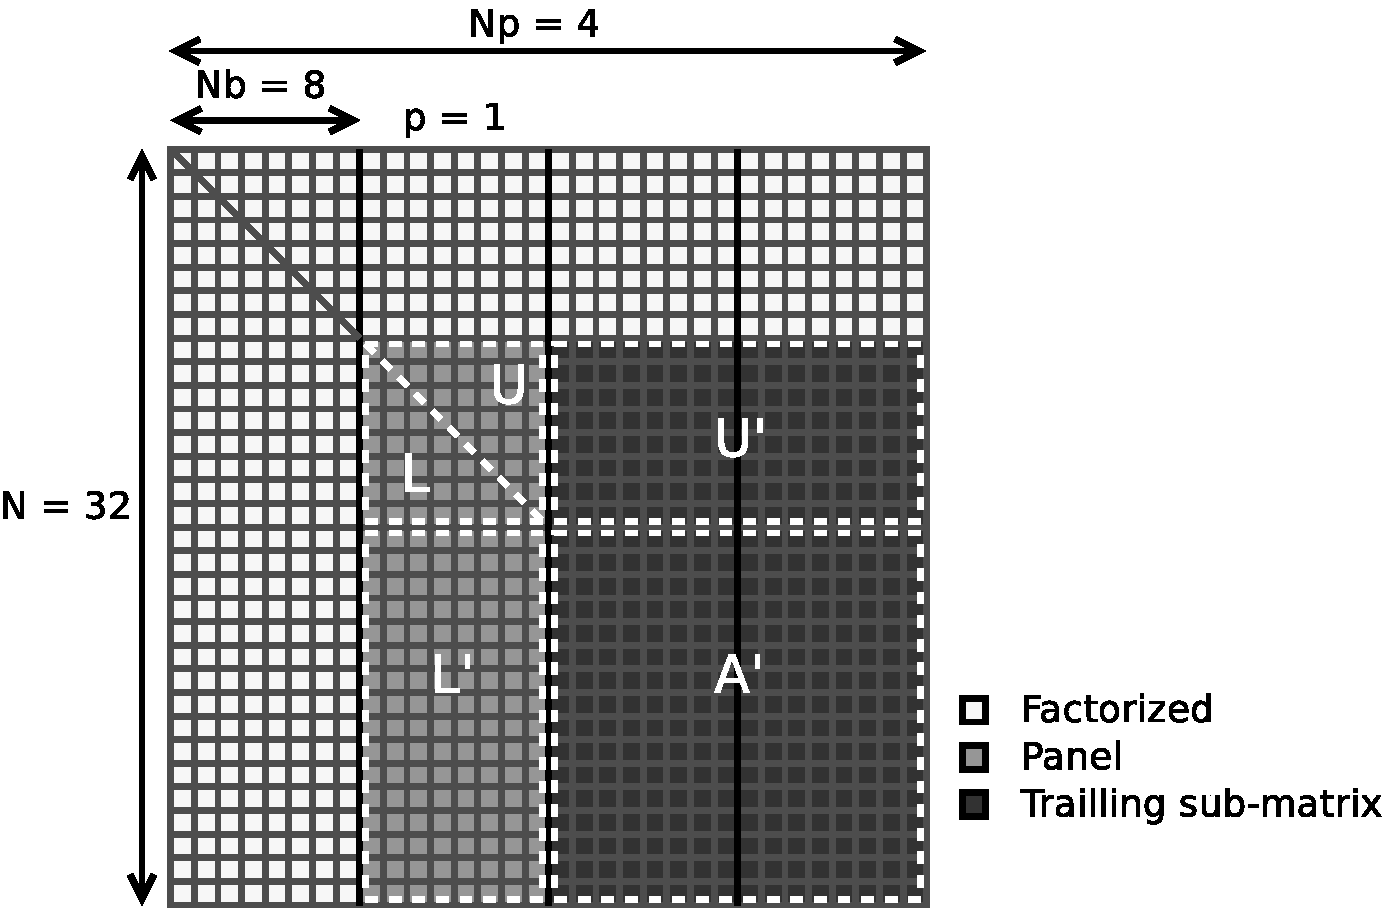
\includegraphics[width=0.9\textwidth]{figures/panel_matrix_bw.pdf}
\caption{LU decomposition at step $p$ on panel-blocked matrix \label{fig:matrix}}
\end{figure}

 
At each step $p$, the panel factorization is performed on the $p_{th}$ panel. Such a panel factorization consists in a loop of $n_b$ iterations. At each iteration $i$ ($p*n_b \leq i < (p+1)*n_b$), a search for the maximum of the $i_{th}$ column is performed, then its row is swapped with the $i_{th}$ row.
Then, a BLAS \textit{scal} routine is applied on the column $i$. It consist to divide all the element of the column $i$ by the selected pivot (Figure \ref{fig:panel} show the different parts of the panel).
After that, the trailing sub-panel is updated with an outer product - so called \textit{ger} according to the BLAS reference -. The panel factorization produces an array of size $n_b$ containing the pivots selected, we note $ipiv$ this array. For each index $x$ of the array $ipiv$, the row $(p*n_b + x)$ will be swapped with the row $(ipiv[x])$.
Mathematically, the panel factorization can be expressed as follows:\\
\begin{tabbing}
For \= $k$ from $1$ to $nb$\\
\> Search for a pivot, do pivoting then store index\\
\> For \=$i$ from $k+1$ to $n$    /*scal operation*/\\
\>\> $a_{i,k} = a_{i,k}/a_{k,k}$\\
\> For \=$i$ from $k+1$ to $nb$   /*ger operation*/\\
\>\> For \=$j$ from $k+1$ to $nb$\\
\>\>\> $a_{i,j} = a_{i,j}-a_{i,k}*_{k,j}$\\
\end{tabbing}

\begin{figure}[!ht]
\centering
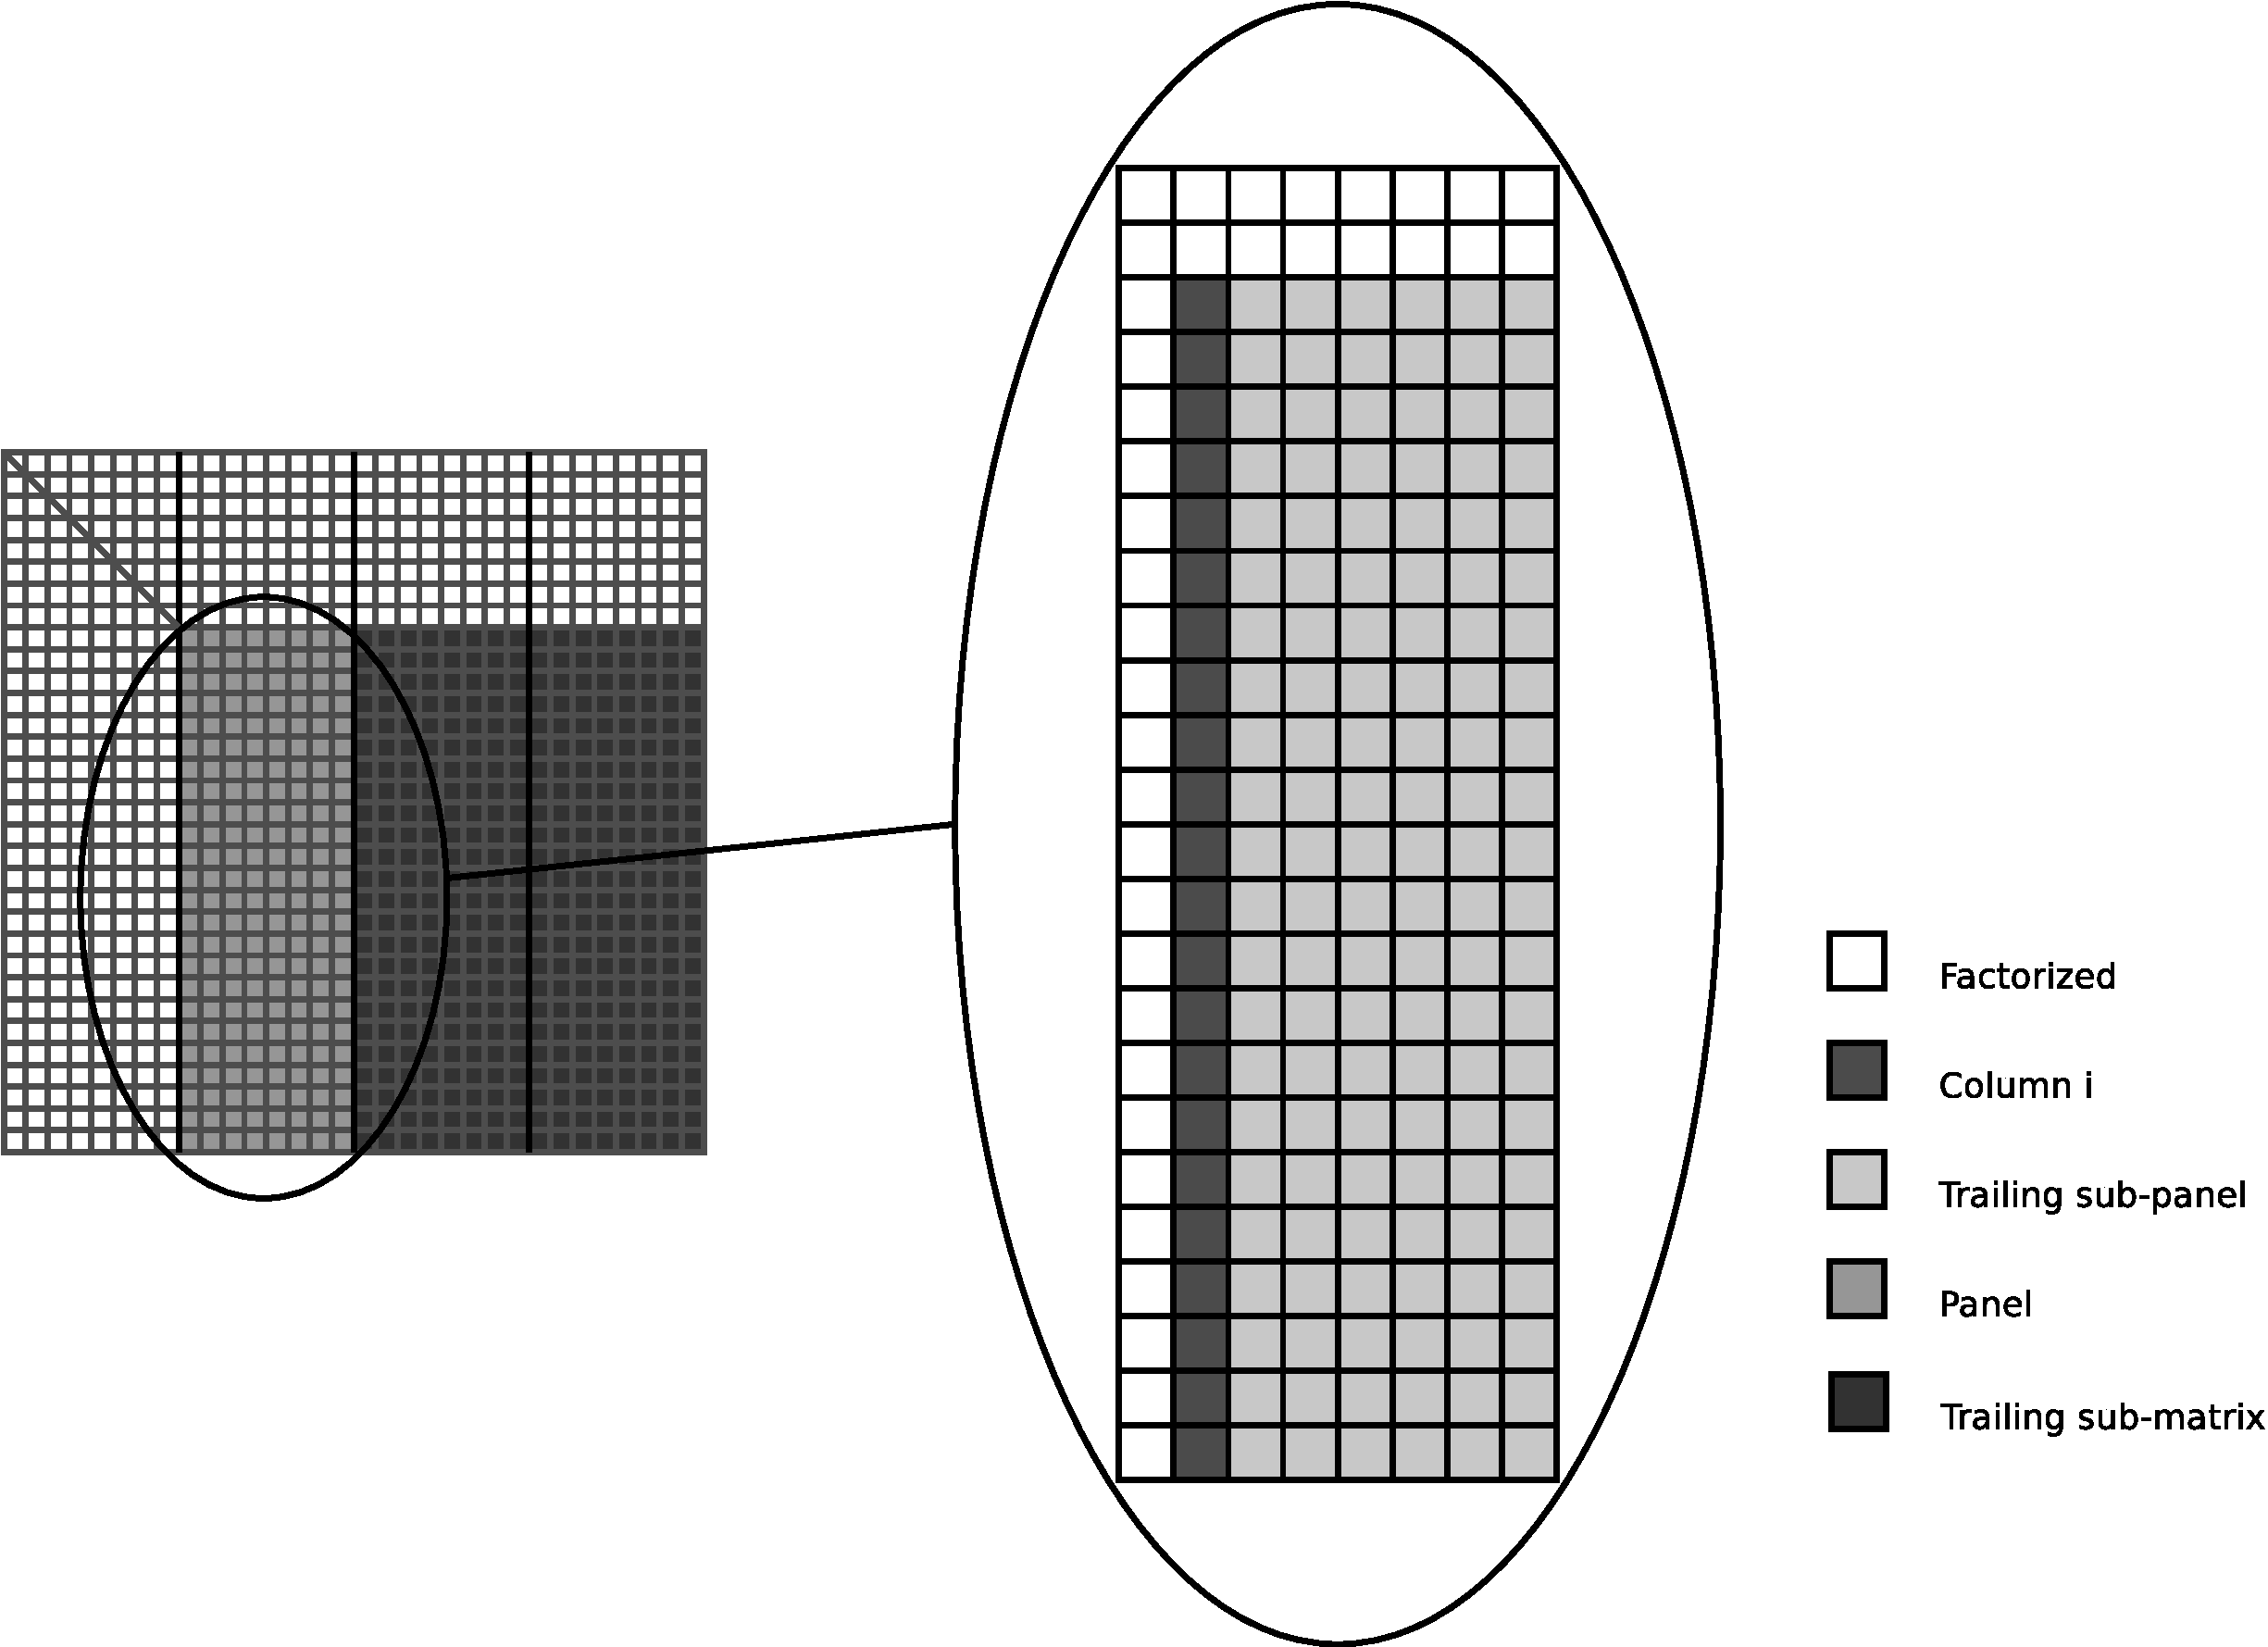
\includegraphics[width=0.8\textwidth]{figures/panel.pdf}
\caption{Second iteration of panel factorization (after swap)\label{fig:panel}}
\end{figure}

Once the $p_{th}$ panel is factorized, the subsequent trailing sub-matrix is updated. This update depend on the panel factorization. It takes as entry the pivot information and then applies the permutations on the whole trailing sub-matrix. Once the swap have been performed on the trailing sub-matrix, the $n_b$ block row corresponding to the eliminated rows (block $U'$ in Figure \ref{fig:matrix}) is updated. For that, the following equation must be solved:
\begin{center}
$U'^{(k)} = U'^{(k+1)}*L$
\end{center}
Which is equivalent to:
\begin{center}
$U'^{(k+1)} = U'^{(k)} / L$
\end{center}
To solve this equation, we can use the BLAS routine \textit{trsm}. The block $U'$ obtained is then multiplied with the block $L'$ and the resulting matrix is subtracted from the matrix $A'$:
\begin{center}
$A'^{(k+1)} = A'^{(k)} - L'^{(k+1)}*U'^{(k+1)}$
\end{center}
This operation is performed with the BLAS routine for matrix multiplication \textit{gemm}.


\section{Task Flow LU Decomposition over Runtimes \label{task_flow_lu}}
We consider the problem of writing the LU decomposition algorithm as a task flow model in order to be executed over runtime systems (particularly on \dague). In the case of dense linear algebra, the algorithms have been redesigned to cope with this model. They are expressed in terms of tasks operating on fine grain squares sub-matrices, also called tiles \cite{conf/para/ButtariDKLLT06,ChanEtAl07b}. Figure \ref{fig:tiled_matrix} shows a matrix partitioned into tiles. In \cite{Buttari09}, the authors proposed a new pivoting strategy called \emph{incremental pivoting} based on \cite{Quintana-Orti:2009:ULF} more suitable tile algorithms and achieved high performance by limiting the number of synchronizations. However, this algorithm has been proven numerically unstable \cite{journals/siammax/GrigoriDX11}. In order to achieve better stability, we choose to adapt the partial pivoting algorithm to the task flow model.

\begin{figure}[!ht]
\centering
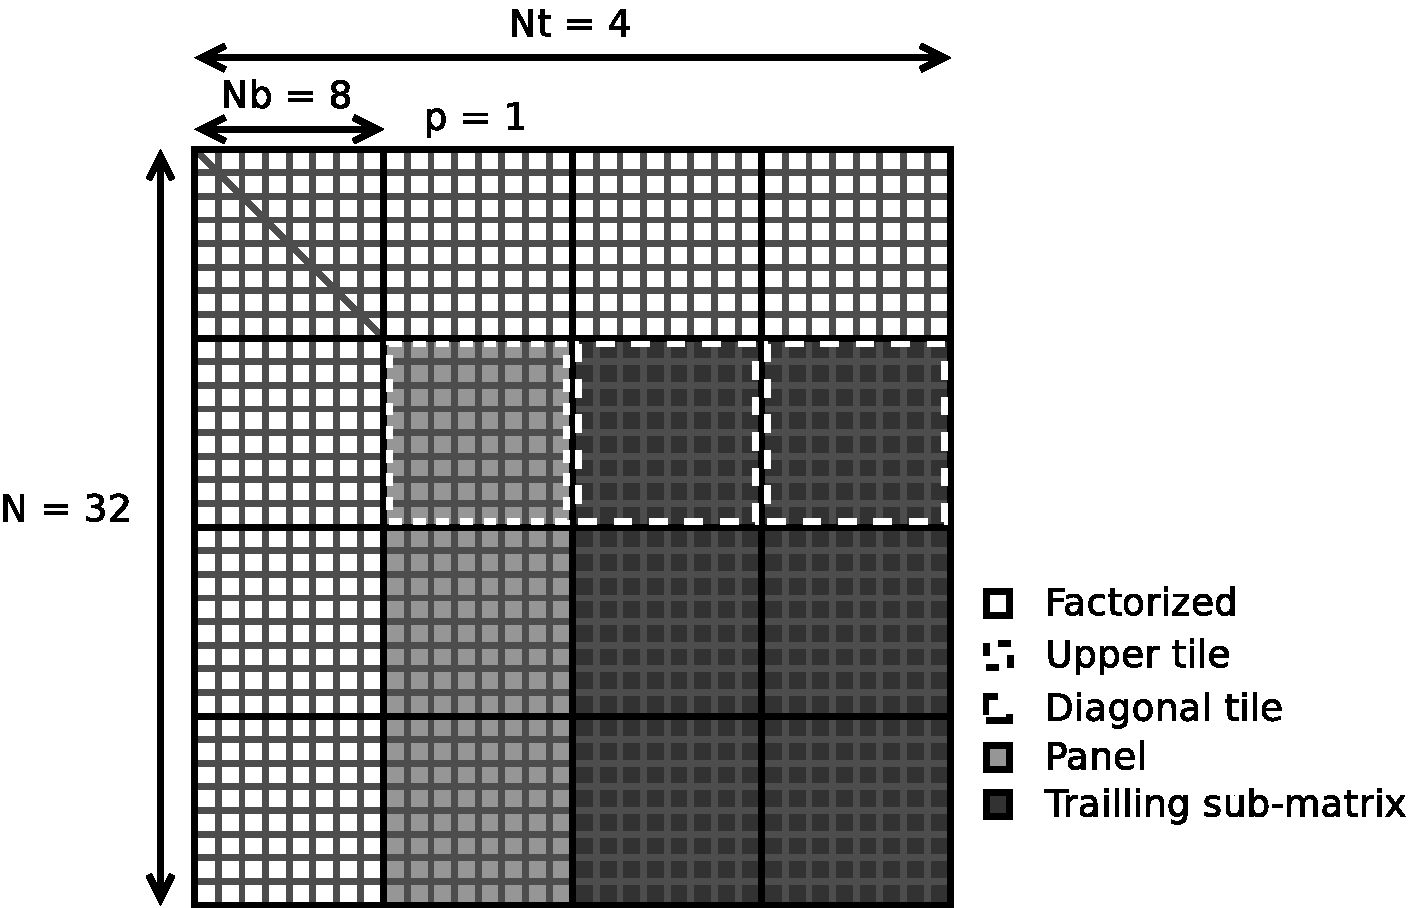
\includegraphics[width=0.9\textwidth]{figures/tiled_matrix.pdf}
\caption{LU decomposition at step $p$ on tiled matrix \label{fig:tiled_matrix}}
\end{figure}

To illustrate the complexity of implementing the algorithm, we consider the pivot research. This research occurs at each column factorization and lies on the critical path of the decomposition. Partial pivoting requires to select the maximum of the elements below the diagonal in the column. Then elements lie on $(n-k)/n_b$ different tiles which may be potentially mapped on a huge number of cores in order to ensure state of the art load balancing techniques. The research induces a synchronization at each column which may overwhelm all potential benefits of tile algorithms and deliver too many tasks to be processed by the runtime.

Another issue with the implementation of the partial pivoting algorithm over the task flow model, is the swapping operation of the update. In fact, after receiving the pivots array from the panel factorization, the upper tile has to send the selected rows to other tiles and receive back the substitute ones. If the swap is done rows by rows, the upper tile may exchange a row with another tile of the panel depending on the numerical values of the pivots. The task flow model can thus no longer be statically build in advance but has then to be dynamically composed. Figure \ref{fig:dynamic} represent a simplified task flow of the sending operation with an automaton. Each time the execution of an algorithm will depend on a value of a data, we will call this phenomenon a \emph{data dependency}. The algorithm which contain data dependencies will be called \emph{dynamic algorithm}. These algorithm may be represented by automatons or others conditional mathematical objects. Unfortunately, almost runtimes supports only static representation of task flow (DAG). Thus, the challenge is to represent a dynamic algorithm with a static representation covering the collection of possibilities. A solution is to create a DAG with a path where all concurrent tasks are sequential and move conditions of transitions to the kernel of the tasks. Figure \ref{fig:static} represent the same dynamic algorithm of Figure \ref{fig:dynamic} with a DAG, we can see that all the tasks are represented sequentially and that the conditions of the dependencies are integrated to the kernels. This transformation may increase tremendously the number of tasks and communications required to execute the algorithm. In the next sections we will present how we reduce the size of this static representation to perform the panel factorization and then update the trailing sub-matrix.

\begin{figure}[!ht]
\begin{minipage}[!ht]{.5\textwidth}
\centering
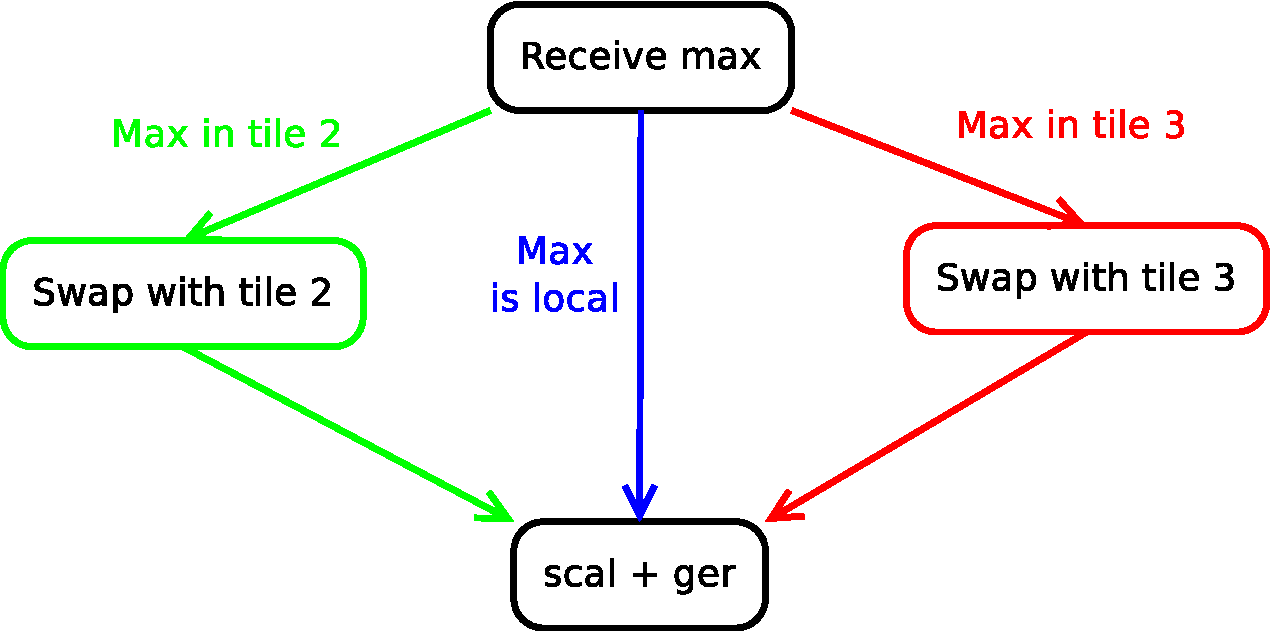
\includegraphics[height=3cm]{figures/dynamic.pdf}
\caption{Dynamic representation of task flow\label{fig:dynamic}}
\end{minipage} \hfill
\begin{minipage}[!ht]{.5\textwidth}
\centering
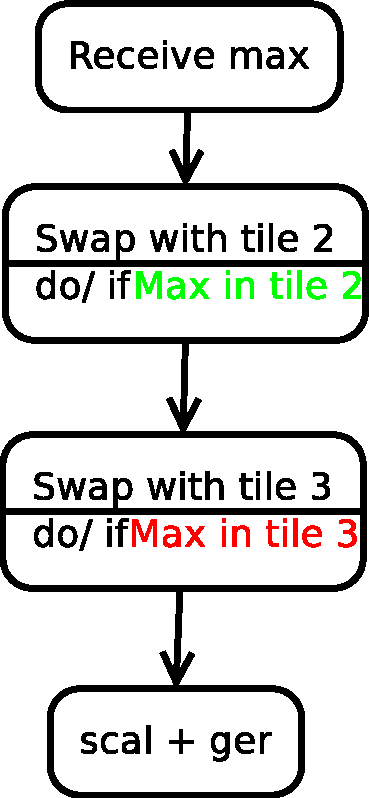
\includegraphics[height=4cm]{figures/static.pdf}
\caption{Static representation of task flow\label{fig:static}}
\end{minipage}
\end{figure}
